\chapter{Proposed Work}
\label{chap:proposed.work}
\section{The Big Picture}
\section{Analytical Proofs}


\section{Results and Discussion}

\begin{figure}[p]
	\centering
	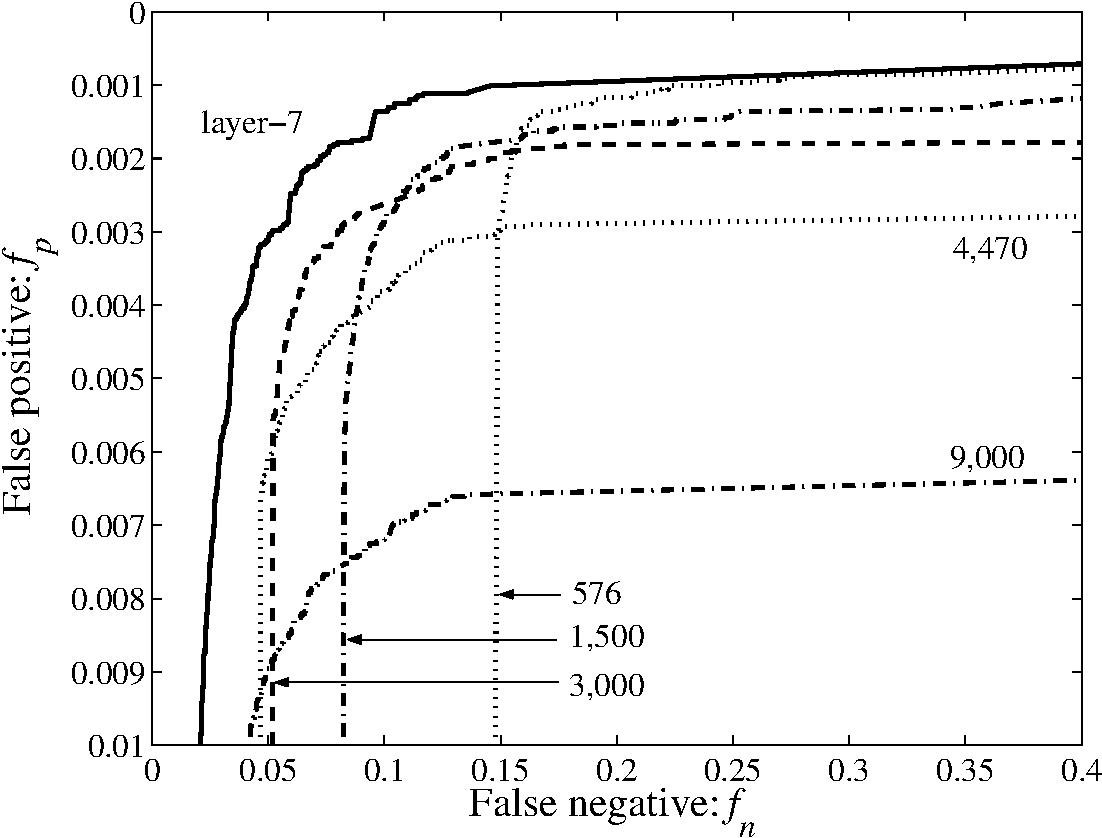
\includegraphics[width=\linewidth]{./figs/roc_TREC}
	\caption[Short version of the caption.]{Example of a figure. This is a long, very long, long long, long caption.  You can give a shorter caption for the ``list of figures" using the square braket symbol.}
\end{figure}


\begin{table}[p]
	\centering
	\caption[Short version of the caption.]{Example of a table. This is a long, very long, long long, long caption.  You can give a shorter caption for the ``list of table" using the square braket symbol.}
	\vspace{\baselineskip}
	\begin{tabular}{l c c}
		\hline
		\hline
		Temperature & Resonant Frequency & Q factor\\
		\hline
		13 mK $\pm$ 1 mK & 16.93 & 811 \\
		40 mK $\pm$ 1 mK & 16.93 & 817 \\
		100 mK $\pm$ 1 mK & 16.93 & 815 \\
		300 mK $\pm$ 1 mK & 16.93 & 806\\
		500 mK $\pm$ 1 mK & 16.93 & 811\\
		800 mK $\pm$ 5 mK & 16.93 & 814\\
		1000 mK $\pm$ 5 mK & 16.93 & 806 \\
		\hline
		\hline
	\end{tabular}
\end{table}

\section{Chapter Summary}